\section{Linguistic analysis}

\subsection{Manual analysis}
This section describes manual marking of the use case steps parts on the \emph{City map} project. 
It explains assigning of the \emph{action type} of the step and binding of the \emph{text ranges} and \emph{action parts}.

We will reuse bundled project \emph{City map} and enhance contained use case \emph{Select city on map}. 

Import project \emph{cityMap} from \emph{exampleProjects} directory and open \emph{Select city on map} use case.

Select first use case step. In sentence analysis view set \emph{Action type} to \emph{To system}
becouse step sentence \emph{"The user opens the map web page"} describes communication of actor and system initiated by actor.

\begin{figure}[ht]
  \centering
  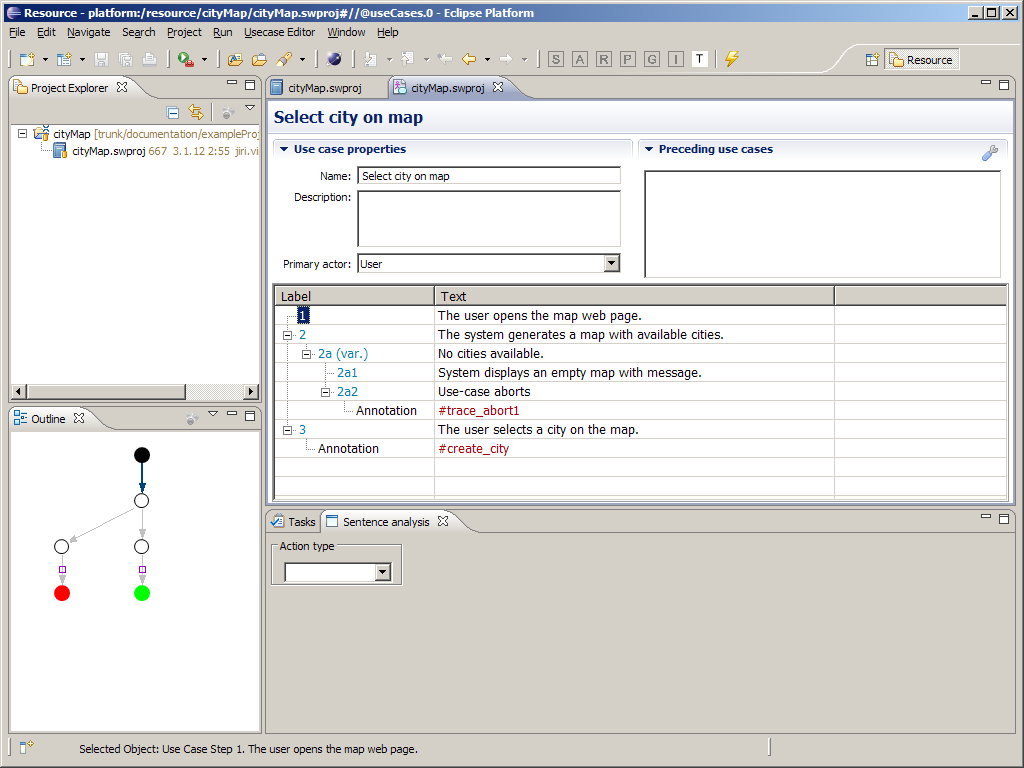
\includegraphics[height=280pt]{images/manual-analysis/step1-action-not-selected}
  \caption{Use case step before action specification}
  %TODO:\label{fig:reprotoolUCEditor}
\end{figure}

Click on the first use case step and notice that boxes in \emph{Sentence analysis view} appeared and three icons in application toolbar got enabled.

\begin{figure}[ht]
  \centering
  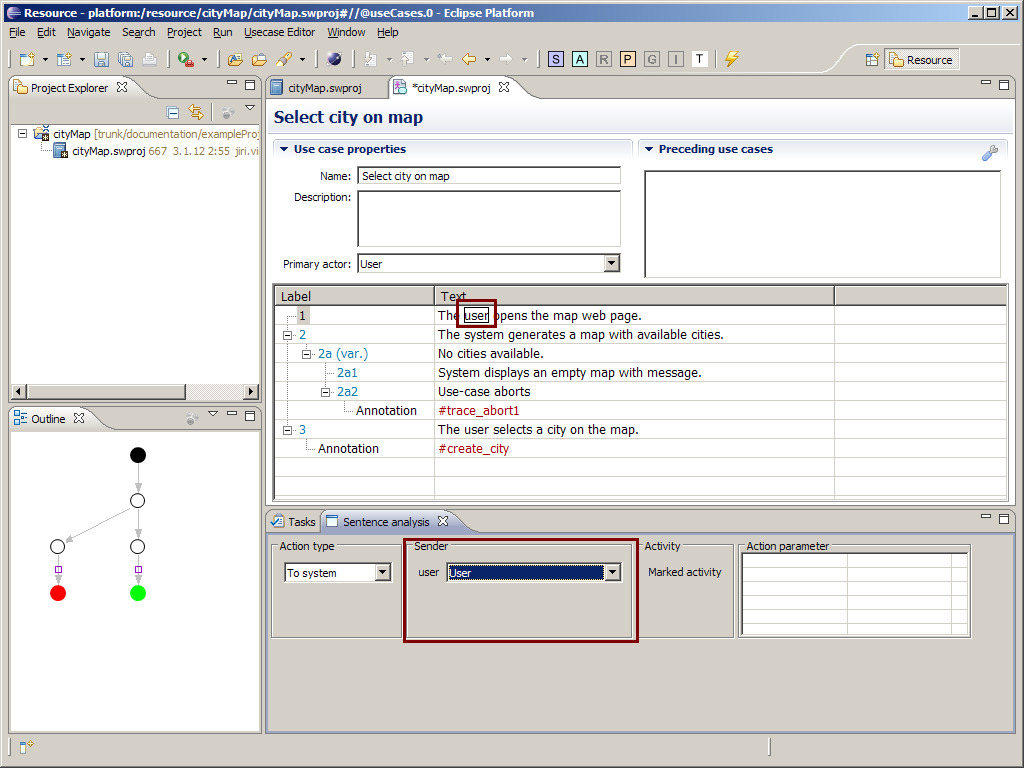
\includegraphics[height=280pt]{images/manual-analysis/step1-action-selected}
  \caption{\emph{To system} action specified}
  %TODO:\label{fig:reprotoolUCEditor}
\end{figure}

Click into second column, select with mouse word "user" and click on "S" toolbar button. Border appears around the word and \emph{Sender} box in \emph{Sentence analysis view} now contains word "user". We call this \emph{textrange} selection. Now select in \emph{Sender} combobox item \emph{"User"}. This combobox is filled with actors contained in project.

\begin{figure}[ht]
  \centering
  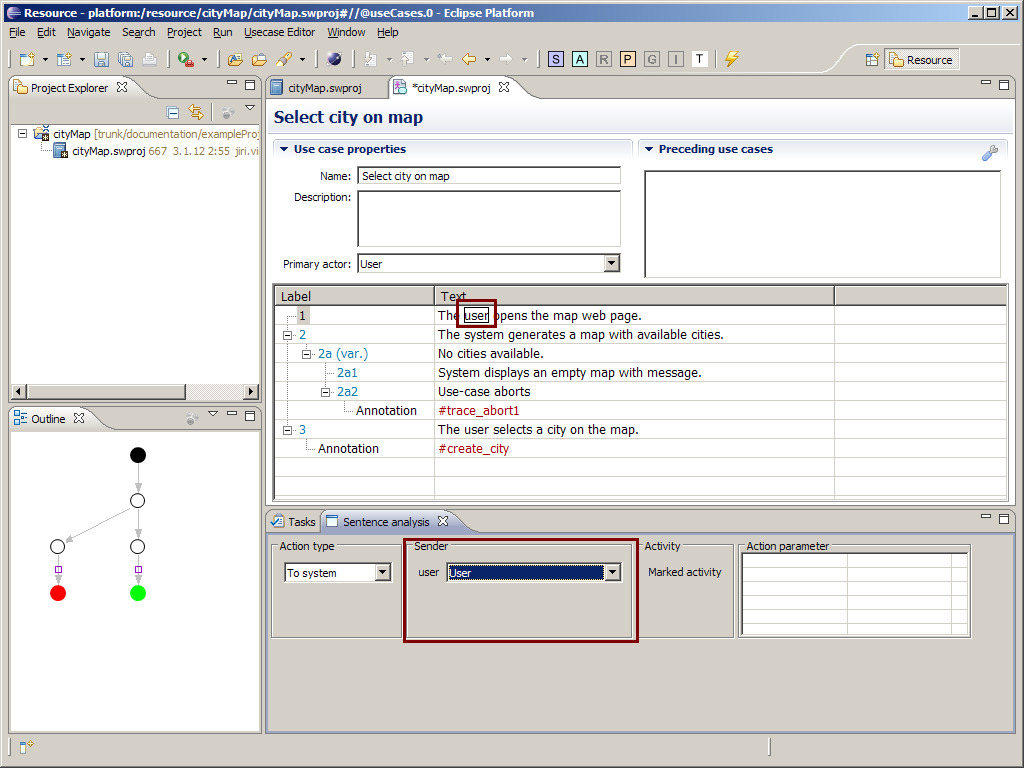
\includegraphics[height=280pt]{images/manual-analysis/step1-sender-selected}
  \caption{\emph{Sender} selected}
  %TODO:\label{fig:reprotoolUCEditor}
\end{figure}

Similarly one can mark \emph{Activity} and \emph{Action parameters}. Box for the \emph{action parameters} allows to add more than one \emph{action parameter} becouse multiple parameters are
allowed in the step sentence. 

Analogous approach allows to mark \emph{Receiver} in the \emph{To system} action ("R" icon), \emph{Goto target} in the \emph{Goto} action ("G" icon) or \emph{Include target} in \emph{Include use case} action ("I" icon). "T" icon allows to "erase" already marked text.

\subsection{Automatic analysis}

Manual analysis can be time consuming. To help user with this tedious task \emph{Reprotool} provides automatic step analysis support. This analysis could be accessed by two different tool-bar commands: Analyse UseCaseStep and Analyse UseCase.

\begin{itemize}
\item {\bf Analyse UseCaseStep}  This command provides linguistic analysis of selected UseCaseStep. From user's point of view it is currently selected sentence in UseCase view. Default icon is at figure \ref{fig:lighting}.
\item {\bf Analyse UseCase}  This command provides linguistic analysis of whole UseCase. From user's point of view this command analyze all sentences in UseCase view. Default icon is at figure \ref{fig:table-lighting}.
\end{itemize}

\begin{figure}[ht]
  \centering
  
\includegraphics[width=15pt]{images/manual-analysis/lightning-16x16}
  \caption{Icon for Analyse UseCaseStep tool-bar command.}
  \label{fig:lighting}
\end{figure}

\begin{figure}[ht]
  \centering
  
\includegraphics[width=15pt]{images/manual-analysis/table-lightning-16x16}
  \caption{Icon for Analyse UseCase tool-bar command.}
  \label{fig:table-lighting}
\end{figure}

Select third use case step \emph{"The user selects a city on the map"}. Click on thunder icon.
GUI may be less responsible for a few seconds while analysis is running.

\begin{figure}[ht]
  \centering
  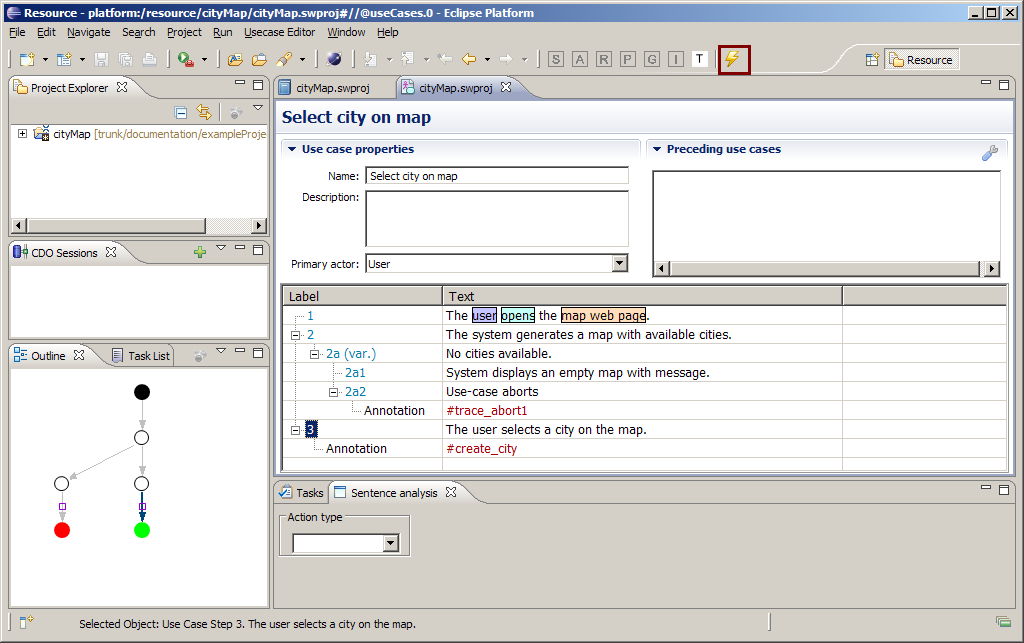
\includegraphics[height=280pt]{images/manual-analysis/step3-automatic-before}
  \caption{Step 3 before automatic analysis run}
  %TODO:\label{fig:reprotoolUCEditor}
\end{figure}

Type of the step should be analysed as \emph{To system} and sender, activity and action parameter
should be filled.

\begin{figure}[ht]
  \centering
  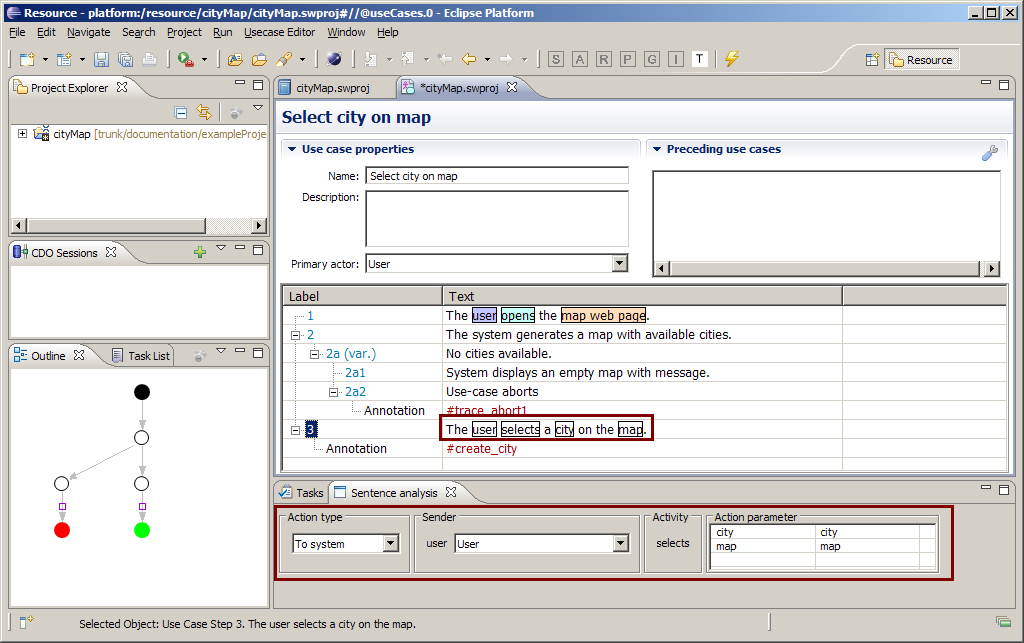
\includegraphics[height=280pt]{images/manual-analysis/step3-automatic-after}
  \caption{Step 3 after automatic analysis run}
  %TODO:\label{fig:reprotoolUCEditor}
\end{figure}

\subsection{Automatic analysis guidelines}

Our goal was to provide linguistic analysis capable of recognition most of the usual natural language sentences located in common use cases. These use cases usually contain computer oriented sentences. Their style and structure depends only on author of use case. Therefore automatic analysis could face really difficult sentences to analyze.

This section provides set of advices for writing use case sentences with no need for manual analysis. Hints how to deal with difficult use case steps are located at the end of this section.

\subsubsection{General advices}
Following set of advices is recommended when use wants to extensively use automatic linguistics analysis. User don't have to follow these advises for using manual analysis. Complexity of UseCaseStepsis only in user's competence, but should keep general rules for writing use cases. 

\begin{itemize}
\item {\bf Fill project properties first} \emph{Reprotool} project contains many important variables, which could be set through project editor. These informations are used during automatic analysis and control its process. Focus also on properties of whole UseCase.

\item {\bf Use common words} It is recommended to use existing commonly used words. Some parts of computer program have more different names, so use the most common one.

\item {\bf Avoid sentence fragments} Automatic analysis gains better results when analyze proper sentences. Some informations are obtained from project context, but these properties are not always sufficient. UseCaseStep sentence is the best place to store step informations.

\item {\bf One action in one UseCaseStep} Always have on mind, that each UseCaseStep can have defined only one action. Complex sentences describing non-atomic actions could not be usually analyzed. Automatic analysis usually analyze only first part of complex sentence. Also use variations and extensions in proper way.

\item {\bf Use meaningful names} Right names and labels quickly remind important informations to user. There is also a lower probability, that they confuse automatic analysis. This advise is more important in bigger projects.

\item {\bf Use basic characters} Linguistics analysis usually use original version of sentence. This means, that sentence string visible to user is used.This string is preprocessed, but not cleared. Linguistics analysis tries to use all informations from this string. When sentence contains set of bad characters, original version is not used. Analysis create safe version of sentence and use this version instead of original version. User can lose full control of analyzed sentence. 
\end{itemize}

\subsubsection{Action types advices}
Sometimes user can want to control linguistics analysis results. \emph{Reprotool} have clearly defined model with specified actions. These actions are strictly defined and unchangeable. Detailed description of automatic action type determination is located in \emph{Reprotool} project documentation.
This section contains only basic tips for each action type and is recommended for common users. Advanced users could make changes to \emph{Reprotool} model and build adjusted version of our project.

\begin{itemize}
\item {\bf Include usecase action} UseCaseStep includes target UseCase. Analysis of this action type is strongly influenced by sentence main verb and specification of target UseCase. Target UseCase must exist in current project. Properly analyzed example sentence is "Include usecase OpenView". 
 
\item {\bf Goto action} This action type is similar to previous action type. Current scenario continues with target UseCaseStep. Properly analyzed example sentence is "Resume with step 2". 

\item {\bf Abort action} Use cases usually contains more terminating steps. Recognition of this step is influenced by sentence main verb. Clear sentence example is "Abort usecase step".

\item {\bf From system action} In this case system interacts with different actor. Subject of this sentence must be system. Example sentence is "System sends message to window". This action is strongly depends on project preferences, e.g. project actors.

\item {\bf To system action} Actor different from system interacts with system. Usually some subsystem prepares something for main system. Usual sentence looks like "Window shows properties to system" or "Selected user fills main-page form".

\item {\bf Internal action} This action type describes situation, where system is subject of sentence and other actors are not important. UseCaseStep usually describes pure system actions. Example sentence is "System throws error".

\item {\bf Unknown action} This is default action type. This type means, that automatic analysis is not able to determine different action type. Read surrounding sections in this manual to avoid these situations.
\end{itemize}

\subsubsection{Accuracy tips}
This section deals with "error situations". User is absolutely sure about UseCaseStep sentence, but automatic linguistic analysis returns different results.

This difference could came from different \emph{Reprotool} model and user's model. For all other situations read following advices.
\begin{itemize}
\item {\bf Project actors} User should review project properties. Insufficient project properties could influence analysis accuracy. Make sure, that all important actors are defined. Best practice is to add default actors "system" and "user".
 
\item {\bf Labels} UseCaseStep and UseCase names or labels are important for targeting these entities. These names should be properly chosen, especially for Goto and Include action types. Best practice is to surround label with quotation marks or apostrophes. E.g. sentence string "Include usecase "Best set of steps"."

\item {\bf Unknown verb} Part of linguistic analysis depends on precomputed statistical models. These models contains big part of all words in current language. It is possible, that sentence contains verb, that is not contained in these models. It is possible, that action type is not recognized (result is Unknown action type), in that case. Easy solution is to use more frequent verb with similar meaning.

\end{itemize}

\subsection{Automatic analysis reports}
This section is focused on more experienced user. Sometimes user needs to know more information about linguistic analysis process. For example, user wants to see individual process parts results. There are two main information views for this purpose. If you are not able to see described views, enable these views from menu Window -> Show view. 

Basics results are shown in Sentence analysis view. This view contains basic informations about sentence and is described in previous sections.

Described analysis results should be sufficient for majority of users. Another way of obtaining more detailed results like constituents determination results are part of benchmark plug-in. See \emph{Reprotool} project documentation for more informations about this feature.

\subsubsection{Console reports}
Console view contains reports from more parts of \emph{Reprotool} application. Lines starting with identification string "[Ling]" are connected with automatic linguistic analysis. These lines usually describe state of analysis or output action type.

\begin{figure}[ht]
  \centering
  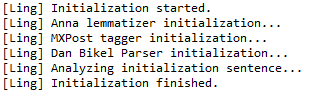
\includegraphics[width=200pt]{images/manual-analysis/console-initialization}
  \caption{Proper console output after linguistic tools initialization.}
  \label{fig:console-initialization}
\end{figure}

\subsubsection{Progress reports}
Initialization of linguistic tools and analysis of each sentence are run as individual job. From users point of view, job is a set of actions that are done with unified way. Result of these jobs are shown in progress view. Each job have its own line and from this line user can access result of this job. This result contains details from main job actions. 

For example, user can see lemma form for all words from current sentence. Example of linguistic analysis job details is shown at figure \ref{fig:progress-detail}.

\begin{figure}[ht]
  \centering
  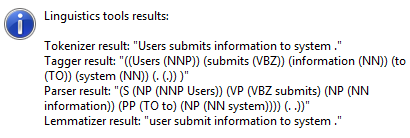
\includegraphics[width=200pt]{images/manual-analysis/progress-detail}
  \caption{Example of linguistic analysis job details.}
  \label{fig:progress-detail}
\end{figure}

There is one special job. It is the initialization job, which is scheduled at startup of  \emph{Reprotool}. This job usually lasts about ten seconds and detail of this job shows actual linguistic tools state. This detail result is actualized when user clicks at OK link of initialization job. Proper detail output can be found at figure \ref{fig:progress-initialization}. There is described state of three external linguistic tools, while parser and lemmatizer should be always running. 

\emph{Reprotool} checks state of these tool during each sentence analysis and in case of error tries to restart these linguistic tools.

\begin{figure}[ht]
  \centering
  
\includegraphics[width=200pt]{images/manual-analysis/progress-initialization}
  \caption{Proper initialization job details dialog.}
  \label{fig:progress-initialization}
\end{figure}


 